\documentclass{scrartcl}[9pt, a4paper]
\usepackage[utf8]{inputenc}
\usepackage[ngerman]{babel}

% Citations
\usepackage[numbers, sort]{natbib}
\usepackage[colorlinks, citecolor=blü, linkcolor=black, urlcolor=green, bookmarks=false, hypertexnames=trü]{hyperref}

% (Computer-)science
\usepackage[ruled, vlined, linesnumbered]{algorithm2e}
\usepackage{amssymb, amsmath}

% Formatting
\usepackage{subcaption}
\usepackage{graphicx}
\usepackage{float}
\usepackage{fancyhdr}

\setlength\parindent{0cm}
\setlength\parskip{0.3cm}

\pagestyle{fancy}
\lhead{
\begin{tabular}{ll}
\end{tabular}
}
\chead{Lösungen Quiz 2}
\rhead{TI-Tutorat}
\lfoot{}
\cfoot{}
\rfoot{\thepage}

% ==============================================================================
% ==============================================================================
\begin{document}

% ______________________________________________________________________________
\section*{Lösung: Aufgabe 1}
\subsection*{Korrekturhinweise}

\begin{itemize}
	\item 2 Punkte für ein Gatter analysis, pro fehlender Zeit (wichtige) [-0.5 Pkt], nicht bezüglich $M$ [-0.5 Pkt]
  \item 1 Punkt für $t_f$
  \item 1 Punkt für korrekte maximal / minimal Zeiten. Delta Fehler jeweils [-0.5 Pkt], Folgefehler ok.
\end{itemize}

\subsection*{Lösung a)}

Berechnung für ein Gatter bezüglich $M$ und $t_0$:

\begin{align*}
	t_p & := t_0 + [0.0, 0.15]                       \\
	t_q & := t_0 + [0.0, 0.15]                       \\
	t_t & := t_q + [0.02, 0.12] = t_0 + [0.02, 0.27] \\
	t_r & := t_p + [0.02, 0.12] = t_0 + [0.02, 0.27] \\
	t_s & := t_t + [0.02, 0.14] = t_0 + [0.04, 0.41]
\end{align*}

Berechnung für 4 Eingangs EXOR bezüglich $M$ und $t_0$:

\begin{align*}
	t_u & := t_s                                     \\
	t_v & := t_s                                     \\
	t_f & := t_u + [0.04, 0.41] = t_0 + [0.08, 0.82] \\
\end{align*}

Berechnung der Zeiten für logische Werte:

\begin{align*}
	t_{min} & := t_f^{min} + \delta         \\
	t_{min} & := t_f^{max} + 2 \cdot \delta \\
\end{align*}

\subsection*{Lösung b)}

Berechnung für ein Gatter bezüglich $M$ und $t_0$:

\begin{align*}
	t_p & := t_0 + [0.2, 0.12]                       \\
	t_t & := t_p + [0.02, 0.12] = t_0 + [0.04, 0.24] \\
	t_r & := t_p + [0.02, 0.12] = t_0 + [0.04, 0.24] \\
	t_s & := t_t + [0.02, 0.14] = t_0 + [0.06, 0.36]
\end{align*}

Berechnung für 4 Eingangs EXOR bezüglich $M$ und $t_0$:

\begin{align*}
	t_u & := t_s                                     \\
	t_v & := t_s                                     \\
	t_f & := t_u + [0.06, 0.36] = t_0 + [0.12, 0.72] \\
\end{align*}

Berechnung der Zeiten für logische Werte:

\begin{align*}
	t_{min} & := t_f^{min} + \delta         \\
	t_{min} & := t_f^{max} + 2 \cdot \delta \\
\end{align*}


% ______________________________________________________________________________
\section*{Lösung: Aufgabe 2}

\subsection*{Lösung \emph{LOADREL}}

\begin{figure}[h]
	\centering
	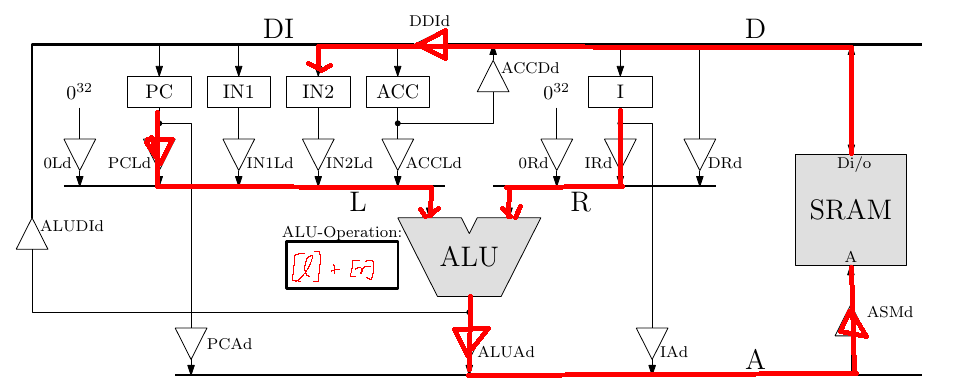
\includegraphics[width=.8\textwidth]{figs/retil1}
\end{figure}


\subsection*{Lösung \emph{STOREREL}}

Nicht realisierbar für $r \neq ACC$. Es werden die Treiber PCDd, IN1Dd, IN2Dd benötigt.

\begin{figure}[h]
	\centering
	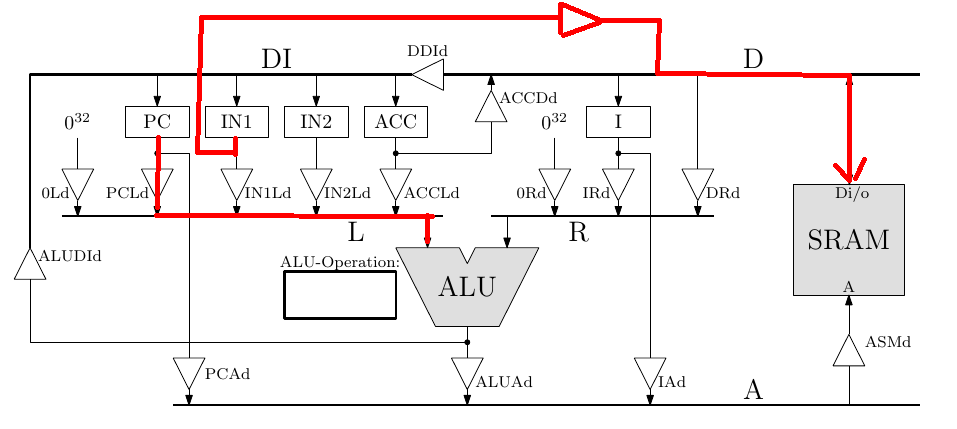
\includegraphics[width=.8\textwidth]{figs/reti}
\end{figure}

\end{document}
